\documentclass{article}

\usepackage{kotex}
\usepackage{graphicx}
\usepackage[affil-it]{authblk}
\usepackage{mathtools}
\usepackage{amssymb}
\usepackage{amsthm}
\usepackage{geometry}
\usepackage{fancyhdr}
\usepackage{braket}
\usepackage{cite}
\usepackage{cancel}
\usepackage{subcaption}
\usepackage{enumitem}
\usepackage{color}
\usepackage{booktabs}
\usepackage{chemformula}
\usepackage{physics}
\usepackage{hyperref}

\newcommand{\vp}{\varphi}
\newcommand{\ve}{\varepsilon}

\newtheorem{theorem}{Theorem}
\newtheorem{definition}[theorem]{Definition}
\newtheorem{example}[theorem]{Example}
\newtheorem{lemma}[theorem]{Lemma}
\newtheorem{axiom}[theorem]{Axiom}
\newtheorem{remark}[theorem]{Remark}
\newtheorem{problem}[theorem]{Problem}
\newtheorem{exercise}[theorem]{Exercise}

\counterwithin{equation}{section}
\counterwithin{theorem}{section}


\geometry{a4paper,left=2cm,right=2cm,top=2.4cm,bottom=2.4cm}

\linespread{1.3}

\title{\textsf{Engine and Refrigerators}}
\author[1]{Written by Eun Taek Kang\thanks{email: etkang03@gmail.com}}
\affil[1]{Department of Physics, Sogang University, Seoul 04107, Korea}

\date{Summer 2025, Sogang University}

\begin{document}

\pagestyle{fancy}
    %... then configure it.
    \fancyhf{}
    % Set the header and footer for Even
    % pages but omit the zone (L, C or R)
    \fancyhead[R]{\textsf{Prof.\ Hyeonjun Baek}}
    \fancyhead[L]{\textsc{Thermal Physics}}
    \fancyfoot[C]{\thepage}
    \fancyfoot[L]{\textbf{Sogang University}}
    \fancyfoot[R]{\textit{Department of Physics}}

\maketitle

\begin{abstract}
    백현준 교수님께서 2025년 1학기에 진행하는 열역학 기말고사 대비를 위해 만든 Note입니다. 이 문서는 Daniel V. Schroeder 저 An Introduction to Thermal Physics의 Chapter 4. Engine and Refrigerators를 다루고 있습니다.
\end{abstract}

\newpage

\section{Heat Engines}

열기관(Heat engines)은 기본적으로 열을 흡수하여 에너지의 일부를 일로 전환하는 기기이다.  

\begin{figure}[h]
    \centering
    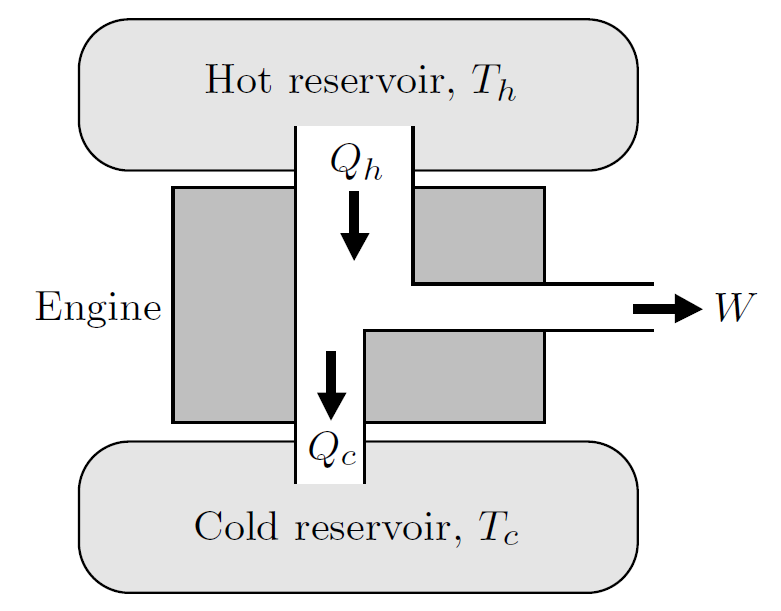
\includegraphics[width=0.35\linewidth]{images/fig1_1.png}
\end{figure}

\noindent
열기관의 구조는 위 그림과 같다. 여기서, 효율성(Efficiency)은 다음과 같이 정의한다.
\begin{equation}
    \ve = \frac{\text{benefit}}{\text{cost}} = \frac{W}{Q_h} = \frac{Q_h - Q_C}{Q_h} = 1 - \frac{Q_C}{Q_h}
\end{equation}
여기서 $W$는 열역학 제1법칙에 의해 전개된다. 또한, 열역학 제2법칙에 의해 engine과 주변의 총 엔트로피는 증가만 하고, 감소하진 않는다. 열기관이 1회 순환하면 엔트로피 변화는 다음과 같다. 
\begin{equation}
    \Delta S_{\text{engine}} = 0, \quad \Delta S_{\text{hot}} = -\frac{Q_h}{T_h}, \quad \Delta S_{\text{cold}} = \frac{Q_c}{T_c}
\end{equation}
동일 state이므로 엔트로피 총 변화는 0이다. 여기서, 열역학 제2법칙을 부등호로 나타내면 다음을 얻는다.
\begin{equation}
    \Delta S_{\text{tot}} = \frac{Q_c}{T_c} - \frac{Q_h}{T_h} \geq 0 \quad \Rightarrow \quad \frac{Q_c}{Q_h} \geq \frac{T_c}{T_h}
\end{equation}
따라서, Efficiency의 최대치는 다음과 같이 결정된다.
\begin{equation}
    \ve = 1-\frac{Q_c}{Q_h} \leq 1-\frac{T_c}{T_h} = \eta
\end{equation}
예를 들어, 고온원이 500K, 저온원이 300K이면, 열효율은 최대 0.4이다. 이처럼, 우리가 최대 열효율을 \textbf{카르노 효율} $\eta$로 정의하자. 열효율을 $\eta$보다 내리는 것은 간단한데, 작동 중에 추가적인 엔트로피를 생성하기만 하면 되기 때문이다. 이상적인 열효율과 다른 경우를 비교해보자. 

\begin{table}[h] \centering
\begin{tabular}{@{}ccc@{}}
\toprule
           & Best efficiency  & Other case                                                      \\ \midrule
열량         & $Q_h$, $Q_c$     & $Q_h ' (= Q_h)$, $Q_c '$                                          \\
온도         & $T_h$, $T_c$     & $T_h ' $, $T_c ' $                                              \\
엔트로피 변화(고온) &
  $\Delta S_h = -\dfrac{Q_h}{T_h}$, $\Delta S_\text{eng.in} = \dfrac{Q_h}{T_h}$ &
  $\Delta S_h = -\dfrac{Q_h}{T_h '}$, $\Delta S_\text{eng.in} = \dfrac{Q_h}{T_h '}$ \\
엔트로피 변화(저온) &
  $\Delta S_c = \dfrac{Q_c}{T_c}$, $\Delta S_\text{eng.out} = -\dfrac{Q_c}{T_c}$ &
  $T_h ' < T_h$일 때, $\Delta S_h + \Delta S_\text{eng.in} > 0$ \\
엔트로피 변화 경향 & 고온, 저온에서 전부 변화 0 & 카르노 X $\rightarrow$ 총 엔트로피 증가, 엔진 $S$ 증가 많이함. \\ \bottomrule
\end{tabular}
\end{table}

우리는 사실 비가역 과정에서 $T_h ' < T_h$인 것도 있고, 엔트로피 증가에 의하여 $Q_c ' / T_c ' > Q_c / T_c$가 성립함을 잘 알고 있다. 따라서 $Q_c ' > Q_c$를 얻는다. 겨론적으로, 같은 양의 열을 가해줬을 때($Q_\text{in} = Q_h$), output heat에서 $Q_c ' > Q_c$가 성립함을 알 수 있다. 따라서, 작동 과정에서 추가적인 엔트로피가 생성되면, 열기관은 비효율적이 된다.


\newpage

\noindent
\textbf{Carnot cycle}

\begin{figure}[h]
    \centering
    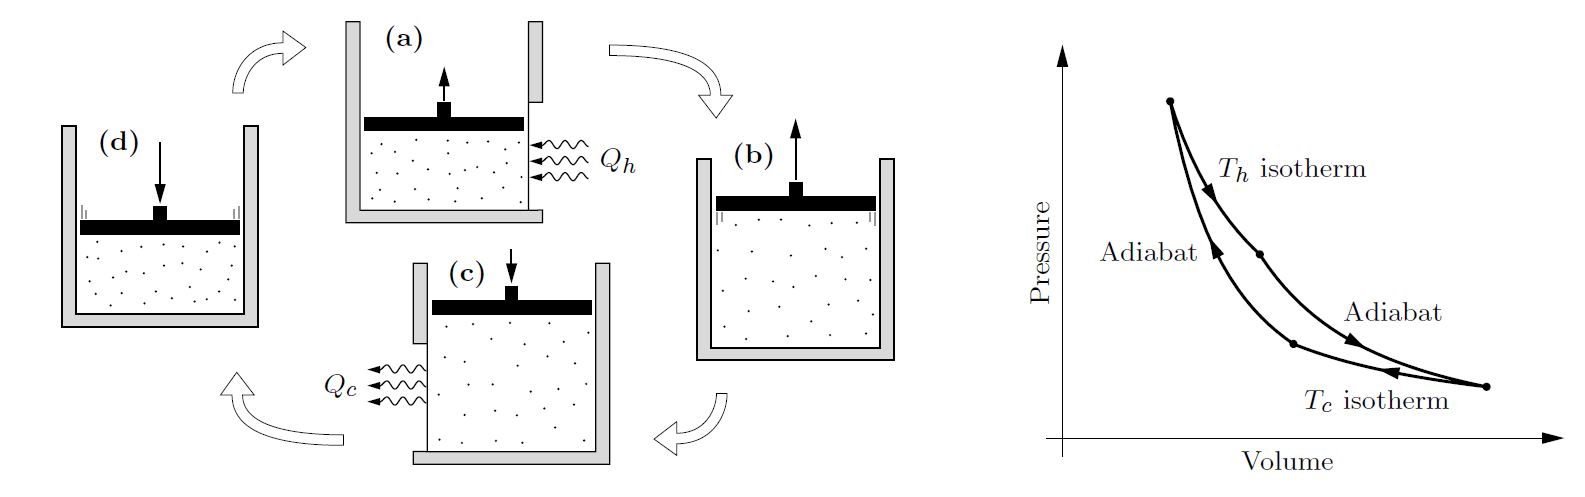
\includegraphics[width=0.95\linewidth]{images/fig1_2.png}
\end{figure}

엔트로피를 생성하지 않는 이상적인 열기관을 어떻게 만들까? 바로 엔진과 열원 간의 온도 $T$가 저온과 고온끼리 서로 같아야한다. 근데, 온도가 같으면 열 흐름이 없어지지 않는가? 그래서 나온 것이 카르노 순환(Carnot cycle)이다. 바로, \underline{엔진 온도를 $T_h$보다 살짝 낮게, 또는 $T_c$보다 살짝 높게 설정해서 등온 팽창/압축} 과정을 거친다. 그리고 기체의 온도를 바꾸는 과정에서 단열 팽창/압축을 사용한다. (열의 출입도 없어서 엔트로피도 변하지 않거든)

카르노 순환은 열효율이 제일 높은 순환을 하는 순환이다. 그러나 \cancel{아쉽게도 매-우} 비실용적이다. 왜냐면, 이건 단열 과정에서 열 흐름이 매우 느린 순환이기 때문이다.

\section{Refrigerator}

냉장고(Refrigerator)는 열기관을 반대로 작동시키는 것이다.  (어떻게 단원 이름이 `냉장고'?ㅋㅋㅋㅋㅋㅋ)

\begin{figure}[h]
    \centering
    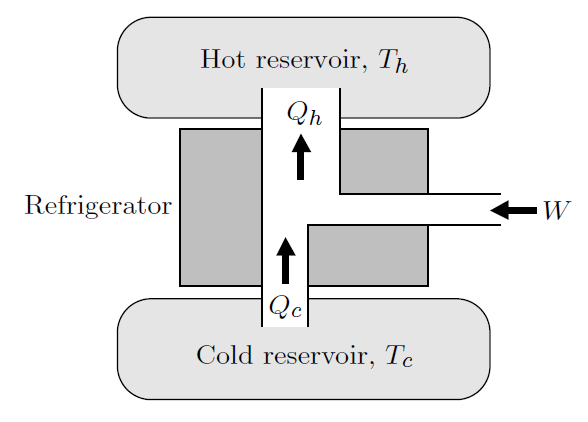
\includegraphics[width=0.4\linewidth]{images/fig2_1.png}
\end{figure}

\noindent
앞서 열기관에선 열효율 $\ve$을 사용했다면, 여기선 성능계수(COP)를 사용하고 다음과 같이 정의한다.
\begin{equation}
    \text{COP} = \frac{\text{benefit}}{\text{cost}} = \frac{Q_c}{W} = \frac{Q_c}{Q_h - Q_c} = \frac{1}{Q_h / Q_c - 1}
\end{equation}
여기서, 열역학 제2법칙에 의해 $\Delta S_\text{tot}$는 다음과 같다.\footnote{열기관과 정확히 반대다!}
\begin{equation}
    \Delta S_{\text{tot}} = \frac{Q_h}{T_h} - \frac{Q_c}{T_c}  \geq 0 \quad \Rightarrow \quad \frac{Q_h}{Q_c} \geq \frac{T_h}{T_c}
\end{equation}
따라서, Efficiency의 최대치는 다음과 같이 결정된다.
\begin{equation}
    \text{COP} \leq \frac{1}{T_h / T_c - 1} = \frac{T_c}{T_h - T_c}
\end{equation}
예를 들어, 고온원이 298K, 저온원이 255K이면, COP는 최대 5.9이다. 따라서 1J의 전기 에너지를 뽑으려고 냉장고에 1+5.9=6.9J의 에너지를 태우게 되는 것이다. COP는 $T_h \approx T_c$일 때, 매우 커진다.

\newpage

\noindent
\textbf{Carnot engine is the most efficient}

\begin{figure}[h]
    \centering
    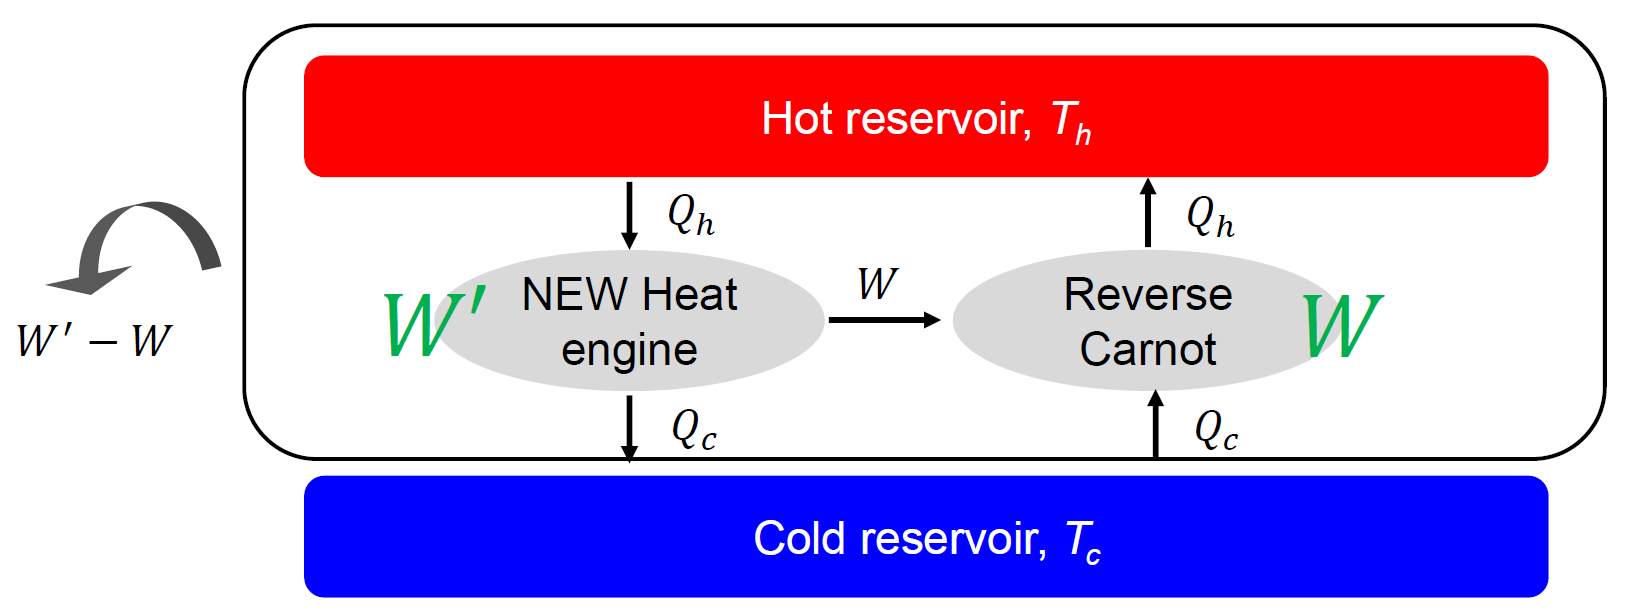
\includegraphics[width=0.75\linewidth]{images/fig2_2.png}
\end{figure}

위 그림에서 $W' - W$는 0보다 클 수 없다. 왜냐하면 다른 변화 없이 단일 온도에서 저수지로부터 유용한 일을 얻는 것은 불가능하기 때문이다. (열역학 제2법칙)

\vspace{2mm} \noindent
\textbf{The efficiency of the Carnot engine}

\begin{figure}[h]
    \centering
    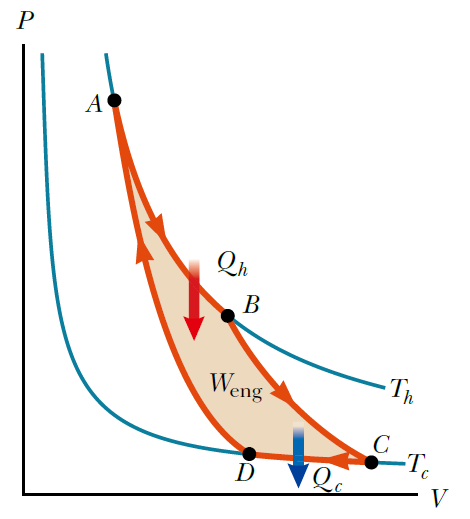
\includegraphics[width=0.4\linewidth]{images/fig2_3.png}
\end{figure}

\noindent
이상기체 상태 방정식이 $\boxed{PV = NkT}$였고, 단열 과정에서 $\boxed{TV^{\gamma - 1} = C}$였음을 기억하자.\footnote{$C$는 당연히 상수이다. $\gamma$는 비열의 비다!! 까먹지 말자.}

\begin{enumerate}
    \item[\textbf{(1)}] A $\rightarrow$ B (등온) : $Q_h = \int_A^B PdV = \int_A^B NkT_h \frac{dV}{V} = NkT_h \ln (V_B / V_A)$
    \item[\textbf{(2)}] C $\rightarrow$ D (등온) : $Q_c = -NkT_c \ln (V_D / V_C) = NkT_c \ln (V_C / V_D)$\
    \item[\textbf{(3)}] B $\rightarrow$ C (단열) : $T_h V_B^{\gamma -1} = T_c V_C^{\gamma -1}$
    \item[\textbf{(4)}] D $\rightarrow$ A (단열) : $T_c V_D^{\gamma -1} = T_h V_A^{\gamma -1}$
    \item[\textbf{(5)}] (3), (4)로부터 $\dfrac{V_B}{V_A} = \dfrac{V_C}{V_D}$이고, (1), (2)는 다음으로 묶어 나타낼 수 있다. $\boxed{\dfrac{Q_h}{T_h} = \dfrac{Q_c}{T_c}}$
\end{enumerate}


\newpage

\section{The Real Heat Engines}

\textbf{Gasolin engine (Otto cycle)}

\begin{figure}[h]
    \centering
    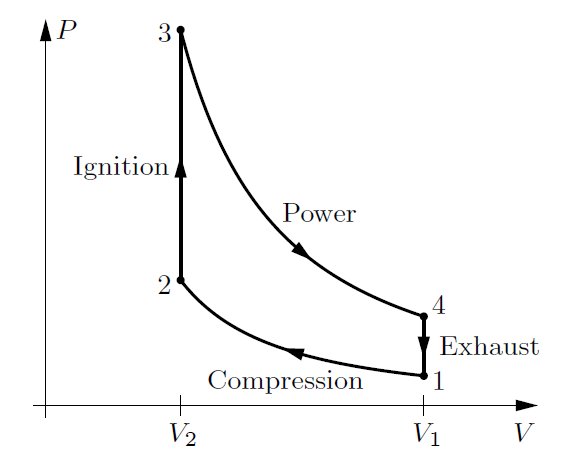
\includegraphics[width=0.45\linewidth]{images/fig3_1.png}
\end{figure}

\noindent
가솔린 엔진은 공기와 기화된 휘발유의 혼합 기체를 연료료 하여 작동하는 열기관이다. 이 열기관이 따르는 사이클을 오토 사이클(Otto cycle)이라 부르는데, 4단계의 과정을 따라 작동한다.

\begin{enumerate}
    \item[\textbf{(1)}] \textcolor{blue}{단열 압축}: 혼합 기체가 실린더 안으로 주입되어 단열 압축한다.
    \item[\textbf{(2)}] \textcolor{blue}{등적 가열}: 스파크 플러그가 혼합 기체에 점화해 온도와 압력을 증가시킨다. 
    \item[\textbf{(3)}] \textcolor{blue}{단열 팽창}: 고압의 기체가 피스톤을 밀어내면서, 기계적 일을 한다. (주 출력!!)
    \item[\textbf{(4)}] \textcolor{blue}{등적 냉각}: 뜨거운 배기가스는 배출되고, 온도와 압력이 더 낮은 새로운 혼합 기체로 교체된다.
\end{enumerate}


\noindent
여기서, 이 열기관의 열효율(efficiency)를 계산하는 과정은 다음과 같다.
\begin{equation}\label{eq:3-1}
    e = 1-\frac{Q_c}{Q_h} =1 - \frac{T_4 - T_1}{T_3 - T_2}, \quad \text{where } \ Q_h = \frac{f}{2} Nk(T_3 - T_2), \quad Q_c = \frac{f}{2} Nk(T_4 - T_1)
\end{equation}
여기서, 단열 압축/팽창 과정에서 다음이 성립한다.
\begin{equation}\label{eq:3-2}
    T_3 V_2^{\gamma -1} = T_4 V_1^{\gamma -1} \quad \text{and} \quad T_1 V_1^{\gamma -1} = T_2 V_2^{\gamma -1}
\end{equation}
(\ref{eq:3-2})를 (\ref{eq:3-1})에 끼워맞출 수 있게 아주 잘 변형해주면 다음처럼 $e$를 표현할 수 있다.
\begin{equation}
    \frac{T_4 - T_1}{T_3 - T_2} = \left( \frac{V_2}{V_1} \right)^{\gamma -1} \quad \Rightarrow \quad \boxed{ e = 1 - \left( \frac{V_2}{V_1} \right)^{\gamma -1}}
\end{equation}
(\ref{eq:3-1})에서 구한 $e$를 단열 과정의 일 관점에서도 구해보자. 단열 과정에선 $W = -\Delta U$임을 기억하자.
\begin{align}
    \text{Expansion} : W_{34} &= \frac{f}{2}Nk (T_3 - T_4)\\
    \text{Compression} : W_{12} &= -\frac{f}{2} Nk (T_2 - T_1)\\
    W_\text{tot} &= \frac{f}{2} Nk (T_3 - T_4 - T_2 + T_1)
\end{align}
따라서, $e$는 다음과 같다.
\begin{equation}
    e = \frac{W}{Q_h} = \frac{(T_3 - T_4) - (T_2 -  T_1)}{T_3 - T_2} = \frac{(T_3 - T_2) - (T_4 - T_1)}{T_3 - T_2} = 1 - \frac{T_4 - T_1}{T_3 - T_2}
\end{equation}

\newpage

예를 들어보자. 이론적으로 공기에 대해 $\gamma = 7/5$이다. 그리고 압축률 ($V_1/V_2$)는 8이라 가정한다.
\begin{equation}
    \ve = 1 - \left( \frac{1}{8} \right)^{7/5 - 1} = 0.56
\end{equation}
열효율은 온도에 대한 항으로 나타낼 수도 있는데, 다음과 같이 표현할 수 있다.
\begin{equation}\label{eq:3-9}
    \begin{cases}
        T_3 V_2^{\gamma -1} = T_4 V_1^{\gamma -1}\\
        T_1 V_1^{\gamma -1} = T_2 V_2^{\gamma -1}
    \end{cases} \quad \Rightarrow \quad e = 1 - \frac{T_1}{T_2} = 1- \frac{T_4}{T_3}
\end{equation}
(\ref{eq:3-9})의 온도비는 카르노 공식의 극단 온도비 $T_1 / T_3$보다 항상 크기 때문에, Otto 엔진은 카르노 엔진보다 덜 효율적이다. 물론, 실제로 열 손실이나 불완전 연소 등의 이유로 Otto의 열효율은 약 20\%이다.

\vspace{3mm}\noindent
\textcolor{red}{\textbf{Warning! : Interpreting of $T$ terms in efficiency}}

우리가 유도했던 otto cycle의 열효율을 잘 보다보면 다음과 같은 의문이 들 수 있다.
\begin{equation}
    e = 1- \frac{T_4 - T_1}{T_3 - T_2} = 1 - \left( \frac{V_2}{V_1} \right)^{\gamma -1}, \quad e = 1 - \frac{T_1}{T_2} = 1- \frac{T_4}{T_3} \quad \Rightarrow \quad \frac{T_4 - T_1}{T_3 - T_2} = \frac{T_1}{T_2} = \frac{T_4}{T_3} \ \ (??)
\end{equation}
우리가 $T$를 통해 $e$를 표현한 것을 보면 오른쪽 등식의 첫 번째 등호가 성립하지 않을까 생각이 든다. 결론부터 말하자면, \textbf{일반적으로 같지 않다!!} (어쩌다 우연히 같아질 순 있어도) 왼쪽 분수식은 가열과 냉각 상황의 온도 변화를 묶어서 비교한거고, 나머지 두개는 개별 단열 상황에서의 온도끼리 묶어 비교했기 때문에 일반적으로 같다고 볼 수 없다. (필자는 처음에 여기를 이해하는데 꽤 오래 걸렸다.) 그냥 온도차의 비율과 온도의 비율은 서로 독립적인 state에 있다고 생각하는게 어쩌면 편할지도..? 

\vspace{2mm}\noindent
\textbf{Diesel engine}

\begin{figure}[h]
    \centering
    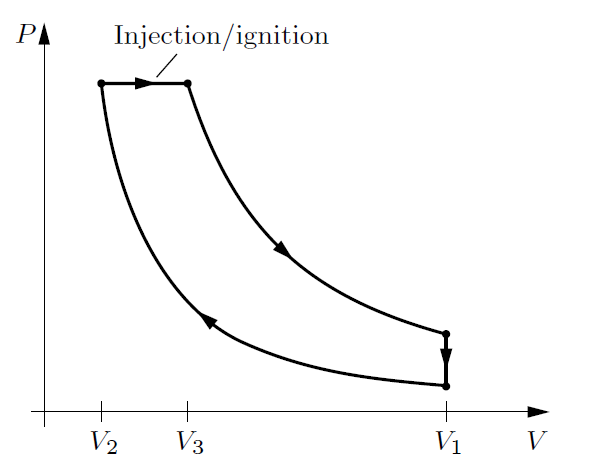
\includegraphics[width=0.425\linewidth]{images/fig3_2.png}
\end{figure}

엔진의 효율을 높이기 위해선 압축비가 더 높으면 되지만, 가솔린은 그러면 압축하다가 지 혼자 i펑! 터져버림!! 그 대안으로 나온게 디젤 엔진(Diesel engine)이다. 공기가 뜨거워지면 연료를 뿌려서 지 혼자 터지는걸 막는다.
\begin{equation}
    \text{efficiency} = 1 - \dfrac{1}{\gamma} \cdot \dfrac{\left( \dfrac{V_3}{V_1} \right)^{\gamma} - \left( \dfrac{V_2}{V_1} \right)^{\gamma}}{\left( \dfrac{V_3}{V_1} \right) - \left( \dfrac{V_2}{V_1} \right)}
\end{equation}
여기서, 압축률은 $(V_1 / V_2)$이고, cutoff 비율은 $(V_1 / V_3)$이다. 이론적으론 디젤 엔진이 otto 사이클보다 열효율이 낮지만, 실제론 압축률이 약 20정도로 매우 높아서 열효율이 otto보다 잘 나온다.

\newpage

\noindent
\textbf{The steam engine}

\begin{figure}[h]
    \centering
    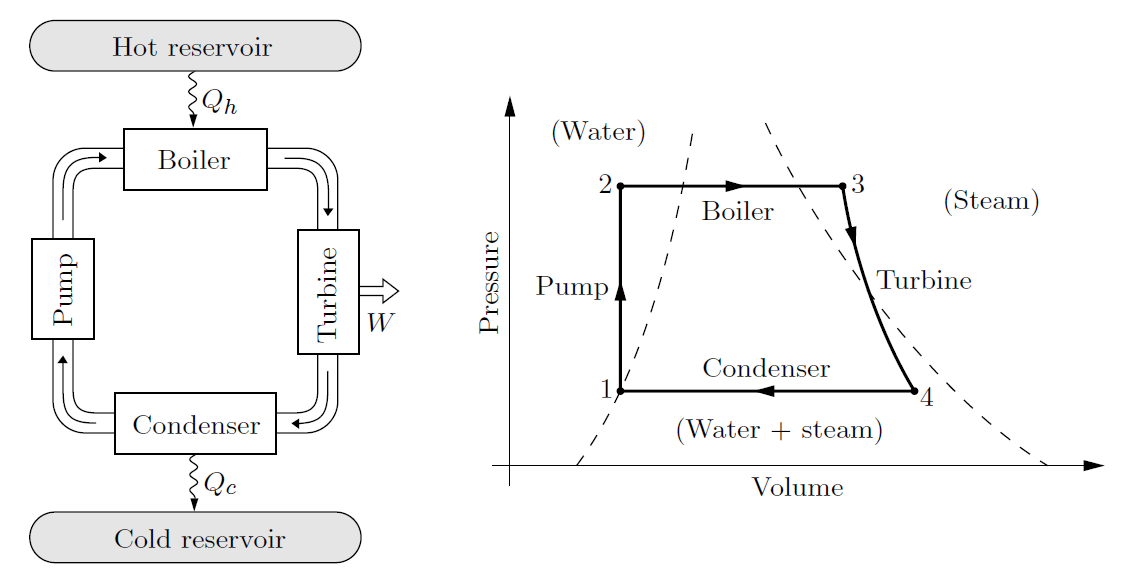
\includegraphics[width=0.7\linewidth]{images/fig3_3.png}
\end{figure}

증기 기관은 우리가 산업 혁명 다루면서 한 번쯤 들어봤을 친구다.. 물과 수증기를 이용해 작동하는데, 작동 원리는 다음과 같다. 이 과정에서 쓰이는 순환 사이클의 이름은 Rankine cycle이다.
\begin{itemize}
    \item (1) $\rightarrow$ (2) : 물은 고압으로 펌프를 통해 압축된다.
    \item (2) $\rightarrow$ (3) : 보일러에서 일정 압력하에 열이 공급된다.
    \item (3) $\rightarrow$ (4) : 수증기는 터빈을 통과하며 단열 팽창하고, 이 과정에서 냉각된다.
    \item (4) $\rightarrow$ (1) : 부분적으로 응축된 유체는 콘덴서에서 더 냉각된다.
\end{itemize}

\noindent
\textbf{Phase diagram of water}

\begin{figure}[h]
    \centering
    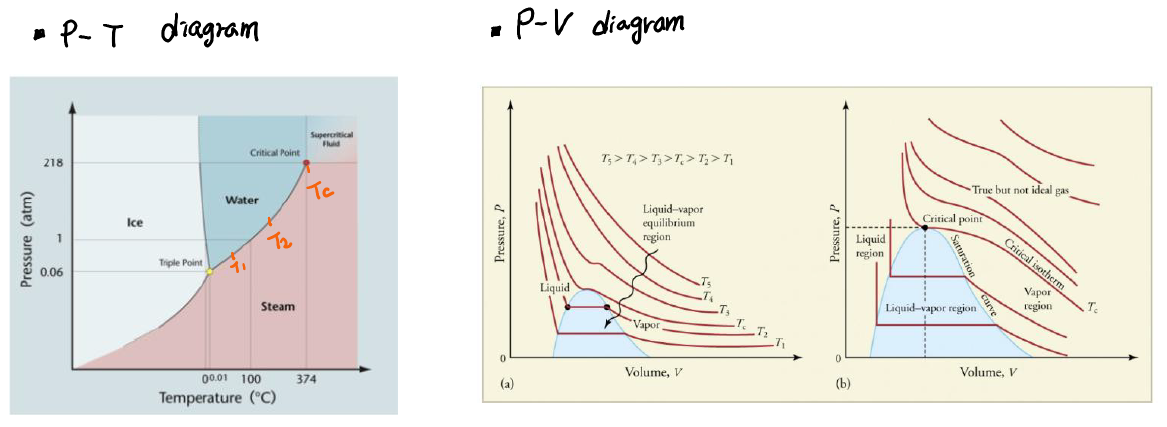
\includegraphics[width=0.85\linewidth]{images/fig3_4.png}
\end{figure}

\noindent
물의 여러가지 상(phase)에 따라서 열기관에 쓰일 때 성질들이 달라잔다. 실제로 증기 기관도 두 가지 상의 물을 쓰고 있으니까. 엔탈피의 식이 $H = U + PV$였다는 것을 기억하자.\footnote{자세한 얘기는 Chapter 5에서 진행한다.} 등압 조건 하에선 $\Delta Q = \Delta H$이다.
\begin{equation}
    e = 1 - \frac{Q_c}{Q_h} = 1 - \frac{H_4 - H_1}{H_3 - H_2} \approx 1 - \frac{H_4 - H_1}{H_3 - H_1}
\end{equation}
이다. $H_2 \approx H_1$이 성립하는 이유는 간단하게 아래와 같다.
\begin{equation}
    \Delta H_{21} = \Delta U + P \Delta V + V \Delta P \approx V \Delta P
\end{equation}
이 페이지는 그냥 간단히 원리정도만 알아둬도 되지 않을까...!

\newpage

\section{The Real Refrigerator}

\begin{figure}[h]
    \centering
    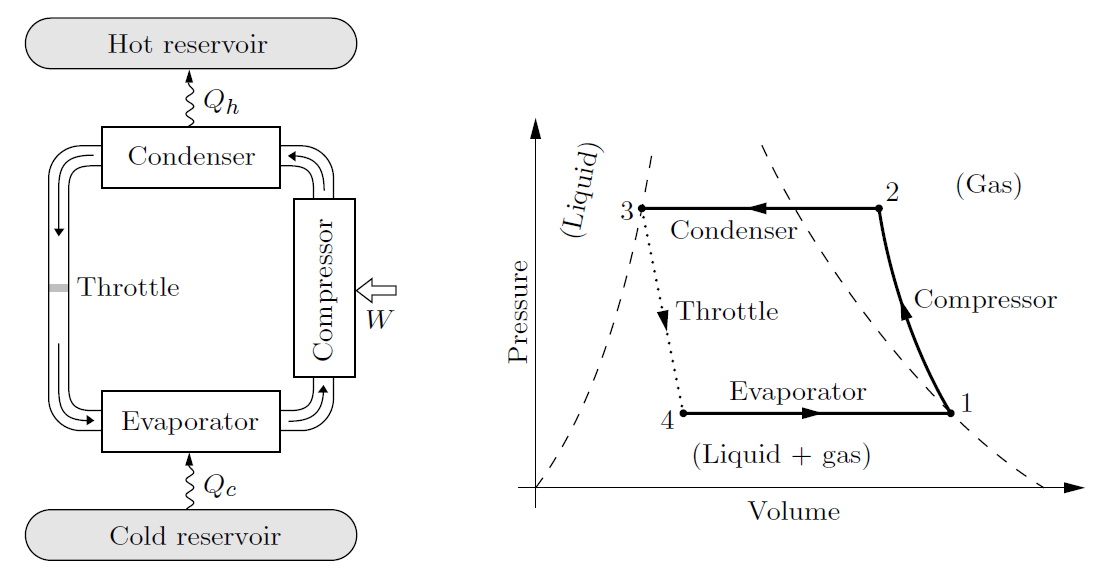
\includegraphics[width=0.75\linewidth]{images/fig4_1.png}
\end{figure}

아까 냉장고는 열기관의 역작용이라 했으니, 실재 냉장고는? 실재 열기관의 사이클인 Rankine 사이클의 역작용과 거의 비슷할 것이다. 작동 물질은 냉매(프레온, HFC)같이 끓는점이 낮은 친구들이어야 하고..
\begin{itemize}
    \item (1) $\rightarrow$ (2) : 냉매는 단열 압축되어 압력과 온도가 올라간다.
    \item (2) $\rightarrow$ (3) : 냉매가 열을 방출하면서 서서히 액화된다.
    \item (3) $\rightarrow$ (4) : \textcolor{blue}{스로틀 밸브}를 통해 냉매가 압력, 온도 낮추며 팽창
    \item (4) $\rightarrow$ (1) : 냉매가 열을 흡수하면서 다시 기체로 증발 (냉각효과 발생)
\end{itemize}

\noindent
\textbf{The Throttling Process}

\begin{figure}[h]
    \centering
    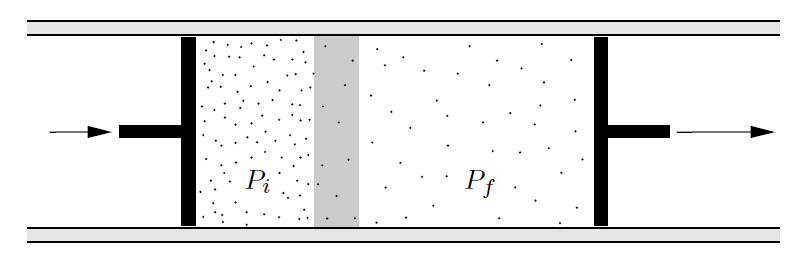
\includegraphics[width=0.55\linewidth]{images/fig4_2.png}
\end{figure}


\end{document}